%----------------------------------------------------------------------------------------
%	Section: Viewer Features
%----------------------------------------------------------------------------------------
\section{Viewer Features}

\begin{figure}[h]
    	\centering
    		\includegraphics[width=1\textwidth]{pics/SurfacesAI.png}
    	\caption[Viewer Features]{There are pages (right) for each feature in the viewer.}
    	\label{fig:featureMenu}
   \end{figure}
	
The feature pages show a list of the respective features, the properties of the selected feature from this list, and some actions for this feature.
For surfaces, annotations, and bookmarks it is possible to group them, as described in Section~\ref{sec:grouping}.
%----------------------------------------------------------------------------------------
%	SubSection: Surfaces
%----------------------------------------------------------------------------------------
\subsection{Surfaces}
\label{sec:surfaces}

The listing shows all surfaces in the scene. You can classify them in any group and subgroup layers, described in Section~\ref{sec:grouping}.
You can select a surface by clicking on the surface's name, which turns its color to green. Or you can set ``PickSurface'' in the actions menu (Figure~\ref{fig:Interactions}), press CTRL+LMB and pick the surface in the main view. Then you can see the surface's properties in the properties panel and use the actions in the actions panel. 
It is also possible to select multiple surfaces by clicking the square icon in front of each surface. The selected surfaces have a green square in the list. The multiselection is used to move one ore more surfaces from one group to the active group.
Under the surface's name is a little menu:
\begin{itemize}
	\item \textit{FlyTo}: A click on the button triggers a FlyTo animation.
	\item \textit{openFolder}: Opens the folder where the scene file resides.	
	\item \textit{Cloud}: Creates new kd-tree files.	
	%\item \textit{portable}: This creates a folder hierarchy as used in the old viewer version. A scene file is created and the surfaces are
  %copied to the surface folder.
	\item \textit{Toggle Visible}: Toggles the surface visible/invisible.	
	\item \textit{Toggle IsActice}: You can only pick on active surfaces (explore center, annotations, ...).
	
\end{itemize}

\begin{figure}[h]
    	\centering
    		\includegraphics[width=1\textwidth]{pics/SurfaceTranslation.png}
    	\caption[Surface Translation]{Translation of the selected surface along the axes of the coordinate system.}
    	\label{fig:surfaceTranslation}
   \end{figure}

For each selected surface there are several panels as shown in Figure~\ref{fig:featureMenu} A to E. 

In the surface properties panel (Figure~\ref{fig:featureMenu} A) some adjustments are possible:
\begin{itemize}
	\item \textit{Name}: The surface's name. You can change it in the text field and press ``enter''.
	\item \textit{Visible}: The surface is visible (checked) or not (unchecked).
	\item \textit{Active}: The surface is active (checked) or not (unchecked). You can only pick on active surfaces.
	\item \textit{Priority}:  Often multiple surfaces are available for a certain area on the planet surface. These surfaces represent the same piece of ground and typically overlap. This parameter allows you to assign a priority to a surface to tell the graphics card which surface should be rendered in front. Lower numbers mean a higher priority in rendering, with 0 being the highest priority. You can also give the highest priority surface a ranking of, for instance, 0.1 (= 10cm) to make annotations more visible. The priority can be dynamically changed via the surface properties so you can try out what works best.
	\item \textit{Quality}: 
	\item \textit{TriangleFilter}: Excludes triangles with edges bigger than the entered value.
	\item \textit{Scale}: 
	\item \textit{FillMode}: You can switch between solid/ wireframe/ point rendering of the geometry.
	\item \textit{Scalars}: Select an attribute layer.
	\item \textit{Textures}: Select a texture layer.
	\item \textit{Cull Faces}:
	\item \textit{Set Homeposition}: You set a new camera position for FlyTo.
\end{itemize}

The surfaces actions (Figure~\ref{fig:featureMenu} B) are described in Section~\ref{sec:leafActions}. \\


You can translate the surface along the north-, east and up axis of the coordinate system, described in Section~\ref{sec:placeCS}. And you can rotate the surface around the up vector of the coordinate system. The Translation panel is shown in Figure~\ref{fig:featureMenu} B and Figure~\ref{fig:surfaceTranslation}. \\

\begin{center}
\colorbox{red}{\parbox{1.0\textwidth}{NOTE: Translation and Rotation only work for surfaces. Annotations, Rovers, the Coordinate System, etc. will NOT move with the surface. You have to transform the surface first!}}
\end{center}

\begin{figure}[h]
    	\centering
    		\includegraphics[width=1\textwidth]{pics/SurfaceColorCorrection.png}
    	\caption[Surface Color Correction]{Contrast-, brightness- and color filters applied on the selected surface.}
    	\label{fig:surfaceColorCorrection}
   \end{figure}

You can apply different color correction filters on the selected surface	(Figure~\ref{fig:surfaceColorCorrection}). \\

\begin{figure}[h]
    	\centering
    		\includegraphics[width=1\textwidth]{pics/SurfaceColorLegend.png}
    	\caption[Surface Color Legend]{A height map visualized by false color mapping.}
    	\label{fig:surfaceColorLegend}
   \end{figure}
	
Within the effort of including more and more meta data for a surface we included the so-called SurfaceAttributes (see Figure~\ref{fig:surfaceColorLegend}),
which are specified in an .opcx file carrying the name of the respective surface.
For now, these surface attributes mainly contain additional layers, which can either be a texture layer or an attribute layer.
Texture layers are just alternative texture maps that can be mapped onto the surface, such as images from different filters or even sensors (spectral image). 
Attribute maps on the other hand present an additional value for each position of a surface. 
If a surface has an .opcx file attached its layers are listed and can be selected in the \textit{Scalars} and the \textit{Textures} combo boxes as part of the surface's property control (Figure~\ref{fig:featureMenu}). 
In the Scalars ColorLegend panel, the color legend can be adjusted (Figure~\ref{fig:surfaceColorLegend}).

%----------------------------------------------------------------------------------------
%	SubSection: Annotations
%----------------------------------------------------------------------------------------
\newpage
\subsection{Annotations}
\label{sec:annotations}

\begin{figure}[h]
    	\centering
    		\includegraphics[width=1\textwidth]{pics/AnnotationsAI.png}
    	\caption[Viewer Features Annotations]{The annotations page.}
    	\label{fig:annoProps}
   \end{figure}
	
The listing shows all annotations in the scene. You can classify them in any group and subgroup layers, described in Section~\ref{sec:grouping}.
You can select an annotation by clicking on the annotation's name, which turns its color to green. Or you can set ``PickAnnotation'' in the actions menu (Figure~\ref{fig:Interactions}), press CTRL+LMB and pick the annotation in the main view. Then you can see the annotation's properties in the properties panel and use the actions in the actions panel. 
It is also possible to select multiple annotations by clicking the square icon in front of each annotation. The selected annotations have a green square in the list. The multiselection is used to move one ore more annotations from one group to the active group.\\
Under the annotation's name is a little menu:
\begin{itemize}
  \item \textit{Toggle}: Toggles the annotation visible/invisible.
	\item \textit{FlyTo}: A click on the button triggers a FlyTo animation.
\end{itemize}

For each selected annotation there are several panels as shown in Figure~\ref{fig:annoProps} A to E. 

The properties of the selected annotation (click on annotation's name) are shown in Figure~\ref{fig:annoProps} A. There you can get information and change some of the settings:
\begin{itemize}
	\item \textit{Geometry}: Shows the annotation mode (described in Section~\ref{sec:drawAnnotation}). This is not changeable retrospectively.
	\item \textit{Projection}: Shows the projection which determines the direction of the picking ray (described in Section~\ref{sec:drawAnnotation}, shown in Figure~\ref{fig:projection}). This is not changeable retrospectively.
	\item \textit{Semantic}: 
	\item \textit{Thickness}: You can change the annotation's line thickness.
	\item \textit{Color}: You can change the annotation's color.
	\item \textit{Text}: You can append a note. Write in the text field and press ``Enter''. The note will appear next to the annotation in the viewer. 
	\item \textit{TextSize}: You can change the textsize.
	\item \textit{Visible}: The annotation is visible (checked) or not (unchecked).
	\item \textit{ShowDnS}: For each annotation with more than three picking points Dip and Strike information (Section~\ref{sec:drawAnnotation}) is available. The DnS is visible (checked) or not (unchecked).
\end{itemize}

The annotations actions (Figure~\ref{fig:annoProps} B) are described in Section~\ref{sec:leafActions}.\\

The measurements tab (Figure~\ref{fig:annoProps} C) contains some information:
\begin{itemize}
	\item \textit{Position}: Shows the position (only for point annotations).
	\item \textit{PrintPosition}: Prints the position in the console window.
	\item \textit{Height}:  The height between the annotation's start and end point.
	\item \textit{HeightDelta}: The height difference between the highest and lowest point of the projected line.
	\item \textit{AvgAltitude}: The average altitude.
	\item \textit{Length}: The sum of direct distances between the picking points.
	\item \textit{WayLength}: The sum of projected distances between the picking points.
	\item \textit{Bearing}: The annotation's bearing.
	\item \textit{Slope}: The annotation's slope.
	\item \textit{Vertical Distance}: The vertical distance between the annotation's start and end point in relation to the up vector of the coordinate system.
	\item \textit{Horizontal Distance}: The horizontal distance between the annotation's start and end point in relation to the north- and right vector of the coordinate system.
\end{itemize}

\begin{figure}[h]
    	\centering
    		\includegraphics[width=1\textwidth]{pics/DnsAI.png}
    	\caption[Viewer Features DnSColorLegend]{Colorcoding of the Dip\&Strike annotations according to their dipping angles.}
    	\label{fig:dnSColorLegend}
   \end{figure}
	
Measurements for the dip and strike annotations are shown in the Dip\&Strike tab (Figure~\ref{fig:annoProps} D and Figure~\ref{fig:dnSColorLegend} D).\\

The color coding of the DnS annotation's discs and arrows is specified by the dipping angle. The color legend's parameters can be adjusted in the
Dip\&Strike ColorLegend tab shown in Figure~\ref{fig:dnSColorLegend} E.

%----------------------------------------------------------------------------------------Import AnnotationGroups
%\subsubsection{Import Annotations from old viewer versions} 
%
%To import annotations from old scene files click the ``browse'' button in the \textbf{ImportAnnotationGroups} section in the Scene Menu (Figure~\ref{fig:StartMenu}). This opens a folder browser dialog, where you can select an old scene file an click ''Open''.
%The annotations are loaded in the same group hierarchy to the ``root'' group.


%----------------------------------------------------------------------------------------
%	SubSection: ViewPlanner
%----------------------------------------------------------------------------------------
%\subsection{ViewPlanner}
%\label{sec:viewPlanner}

%----------------------------------------------------------------------------------------
%	SubSection: Bookmarks
%----------------------------------------------------------------------------------------
\subsection{Bookmarks}
\label{sec:bookmarks}

%\begin{figure}[h]
    	%\centering
    		%\includegraphics[width=0.5\textwidth]{pics/bookmarks.png}
    	%\caption[Viewer Features Bookmarks]{The bookmarks tab.}
    	%\label{fig:bookmarks}
   %\end{figure}
	
Bookmarks enable the user to record a certain camera viewpoint.
To add a new bookmark click the ``+'' button on top of the page. The new bookmark is added to the active group in the bookmarks listing.
To view the bookmark's properties and actions click on the bookmark's name. Clicking the ``house'' button beside the bookmark's name triggers a FlyTo. For multiselection click on the bookmark's square icons.

%----------------------------------------------------------------------------------------
%	SubSection: Bookmarks
%----------------------------------------------------------------------------------------
\subsection{Sequenced Bookmarks}
\label{sec:sequenced_bookmarks}

Sequenced bookmarks can be used to create, view, and record camera flight paths between bookmarks (Figure \ref{fig:seqBookmarks}). Properties like visibility of surfaces, annotations, and scale bars (the \emph{scene state}) are also recorded with bookmarks, and applied during animations.

\begin{figure}[h]
	\centering
	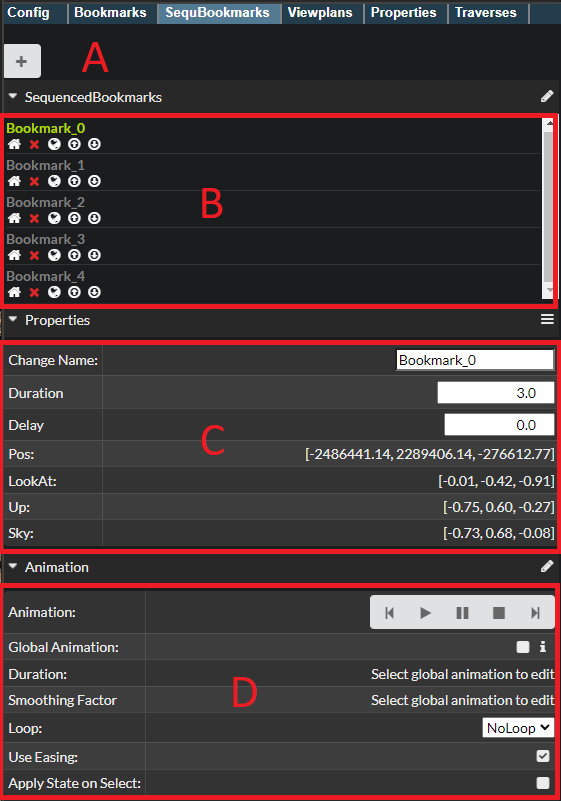
\includegraphics[width=0.5\textwidth]{pics/SequencedBookmarks_tabUpper.PNG}
	\caption[Viewer Features Bookmarks]{The sequenced bookmarks tab.}
	\label{fig:seqBookmarks}
\end{figure}

The scene state includes properties of surfaces, annotations and scale bars. It also includes general viewer settings in the \emph{Config} tab. 

Add bookmarks by clicking on the button with the plus icon at the top (A).

\begin{figure}[h]
	\centering
	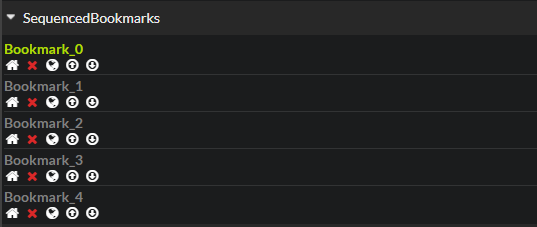
\includegraphics[width=0.8\textwidth]{pics/SequencedBookmarks_list.png}
	\caption[Viewer Features Bookmarks]{The list of all sequenced bookmarks.}
	\label{fig:seqBookmarks_list}
\end{figure}

In the list of bookmarks (B, Figure \ref{fig:seqBookmarks_list}) you can (from left to right) move the camera to the bookmark, delete the bookmark, update the scene state, and move the bookmark up and down in the list. Clicking on the label of a bookmark selects it. The selected bookmark is highlighted in green.

Updating the scene state for an annotation does not update its camera view.

\begin{figure}[h]
	\centering
	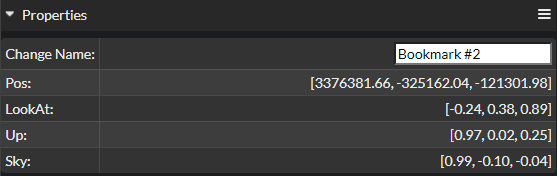
\includegraphics[width=0.8\textwidth]{pics/SequencedBookmarks_properties.png}
	\caption[Viewer Features Bookmarks]{The properties of the selected bookmark.}
	\label{fig:seqBookmarks_properties}
\end{figure}

You can find the properties of the selected bookmark (Figure \ref{fig:seqBookmarks_properties}) below the list of bookmarks (C). Here you can change the bookmark's name.

For each bookmark, you can set two values. The \emph{duration} is the amount of time it takes the camera to move from the previous bookmark to this bookmark. The \emph{delay} determines how long the camera pauses at the bookmark before moving to the next one.

\begin{figure}[h]
	\centering
	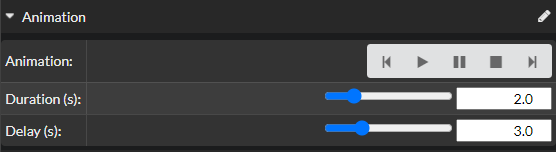
\includegraphics[width=0.8\textwidth]{pics/SequencedBookmarks_animation.png}
	\caption[Viewer Animation]{Animation settings.}
	\label{fig:SequencedBookmarks_animation}
\end{figure}

You can animate the camera according to the list of bookmarks by clicking the play button in the \emph{Animation} section (D). The animation control buttons from left to right: Move to previous bookmark, start camera animation along all bookmarks, pause camera animation, stop camera animation, move camera to next bookmark.

Selecting the checkbox \emph{global animation} has the following effects: 

\begin{itemize}
	\item A spline is used to travel a path along all bookmarks. The smoothing factor determines how smooth the path is. A value closer to zero means that the path hits individual bookmarks more precisely while a larger in general means a smoother path.
	\item The duration is set for the whole animation and cannot be set for individual bookmarks.
	\item The delay for individual bookmarks can not be used.
\end{itemize}

If there are large changes in the scene (and depending on hardware) the animation might not be entirely smooth when proceeding to a new bookmark.

There are three settings for looping: No loop, mirror, and repeat.

If the checkbox \emph{use easing} is selected, the camera animation speeds up in the beginning, and slows down at the end. When global animation is selected, easing is used at the beginning and the end of the whole path. When it is not selected, easing is used for each bookmark.


%\begin{figure}[h]
%	\centering
%	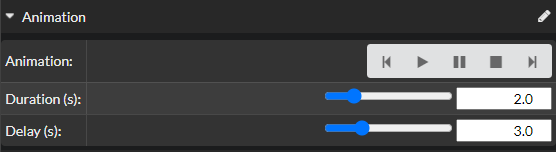
\includegraphics[width=0.8\textwidth]{pics/SequencedBookmarks_animation.png}
%	\caption[Viewer Features Bookmarks]{The animation controls. Buttons from left to right: Move to previous bookmark, start camera animation along all bookmarks, pause camera animation, stop camera animation, move camera to next bookmark.}
%	\label{fig:seqBookmarks_animation}
%\end{figure}


\begin{figure}[h]
	\centering
	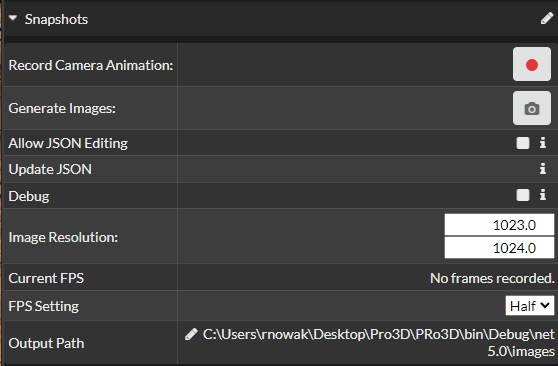
\includegraphics[width=0.8\textwidth]{pics/SequencedBookmarks_tabSnapshots.png}
	\caption[Viewer Features Bookmarks]{Creating images from sequenced bookmarks. Record camera animations as JSON snapshot files (red record button) and start generating images (camera button).}
	\label{fig:SequencedBookmarks_tabSnapshots.PNG}
\end{figure}

In the \emph{snapshots} section (Figure \ref{fig:SequencedBookmarks_tabSnapshots}) you can record camera animations. The red button changes to a \emph{stop} button when you start recording. If you now use the animation controls (D) to animate the camera, the camera movement is recorded. Once you click on the red stop button, a JSON file with the recorded camera animation is saved into the output folder specified in the \emph{Snapshots} section (E). To start rendering images with the saved file, click on the button with the camera icon next to the red record button. PRo3D will start rendering the images in the background.

The following settings are available:
\begin{itemize}
	\item \textbf{\emph{Allow JSON Editing}} There are more options for generating images you can use if you edit the JSON file PRo3D creates (see section \ref{sec:snapshots}). Select this option if you want to edit additional properties in the JSON file (like the field of view) manually. If this option is selected, the JSON file is NOT regenerated when clicking on the \emph{Generate Images} button. This means that settings changed after recording will not be taken into account. Click on the \emph{Update} button if you want to update the JSON file, but be aware that all manual changes will be overwritten. Make sure to backup a JSON file once you have changed it manually, as PRo3D will write over it as soon as you record a new sequence. You can also start the generation process via the command line (Section \ref{sec:CLI}) using an old JSON file. 
	\item \textbf{\emph{Update JSON}} Only available if \emph{Allow JSON Editing} is selected. Updates the JSON file with the current settings. All manual changes to the JSON file are overwritten. 
	\item \textbf{\emph{Image Resolution}} Resolution of output images. Larger images take longer to render.
	\item \textbf{\emph{Current FPS}} Once an animation sequence has been recorded, the FPS of that sequence are displayed here.
	\item \textbf{\emph{FPS Setting}} You can select full or half FPS, the actual FPS depend on the value displayed as \emph{Current FPS}. 
	\item \textbf{\emph{Output Path}} The path where the rendered images will be saved. Click on the path to change it.
\end{itemize}

To record an animation sequence follow these steps (the letters in parentheses refer to figure \ref{fig:seqBookmarks}):

\begin{enumerate}
	\item Add some sequenced bookmarks at different locations using the + button (A).
	\item Set delay and duration to your liking (C). Press play to test your settings (D).
	\item Set image resolution and other snapshot settings (E).
	\item Click on the red record button in the snapshots section (E).
	\item Click on play to start the animation (D).
	\item Wait until the animation is finished.
	\item Click on the red stop button in the Snapshots section (E).
	\item Click on the button with the camera icon (E, \emph{Generate Images}).
\end{enumerate}
%----------------------------------------------------------------------------------------
%	SubSection: Viewer Configuration
%----------------------------------------------------------------------------------------
\subsection{Viewer Configuration}
\label{sec:config}

To edit the viewer properties, select the ``Config'' page.

%----------------------------------------------------------------------------------------Viewer Config
\subsubsection{ViewerConfig} 

A set of major viewer properties can be adjusted:
\begin{itemize}
	\item \textit{Near/Far Plane}: The near- and the far clipping plane are automatically adjusted according to the data to be rendered. The set values are shown in the config panel and can be adjusted afterwards. 
	\item \textit{Navigation Sensitivity}: The navigation sensitivity can also be adjusted by PageUp and PageDown keys. 
	\item \textit{Arrow Length/Thickness}: The arrow length and thickness is set for up- and north vectors, dip and strike vectors and the up- and lookAt vectors in the rover view planner. 
	\item \textit{D+S Plane Size}: The dip and strike measurements plane size, described in Section~\ref{sec:drawAnnotation}
 (Figure~\ref{fig:drawAnnotations}).
	\item \textit{Min/Max Dipping Angle}: The dip and strike measurements dipping angle range. The dipping angle is coded into the color of the disc and arrow of a measurement (Figure~\ref{fig:drawAnnotations}).
	\item \textit{Lod Colors}: The different levels of detail of the surface geometry can be colored in different shades of red.
			This helps to evaluate the export of OPC data.
\end{itemize}

%----------------------------------------------------------------------------------------Coordinate System
\subsubsection{Coordinate System} 

The coordinate system menu shows the position, Up- and North Vector of the coordinate system described in Section~\ref{sec:placeCS}, shown in Figure~\ref{fig:coordinateSystem}.
The Up- and the North Vector are used for the projection measurements (Figure~\ref{fig:drawAnnotations}). Initially the Up Vector's direction is set in the positive z-direction and the North Vector's in the positive y-direction. But you can manipulate the Up Vector manually for different data. Both vectors are computed automatically with picking of a new position for the coordinate system. The north vector is further relevant for bearing measurements. % and the rover placement in the View Planner (see Section 4.6). 

%----------------------------------------------------------------------------------------Camera
\subsubsection{Camera} 

The Camera submenu shows the Location, Forward- and Sky vector of the main camera.


\subsubsection{Frustum}

In this menu the frustum can be adjusted.

\subsubsection{Screenshots}

This menu can be used to create screenshots of the current scene. Click on the button with the camera icon (left) to create a screenshot. Click on the button with the folder icon (right) to open the folder where screenshots are saved. Width and height can be specified in pixels. The output format can be selected as PNG or JPG. Screenshots are saved as \texttt{img} with a number suffix. 

\begin{figure}[h]
	\centering
	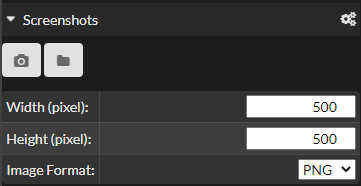
\includegraphics[width=0.6\textwidth]{pics/screenshots.PNG}
	\caption[View Planner]{The screenshots menu. Click on the button with the camera icon (left) to create a screenshot. Click on the button with the folder icon (right) to open the folder where screenshots are saved.}
	\label{fig:screenshots}
\end{figure}



%----------------------------------------------------------------------------------------
%	SubSection: Grouping
%----------------------------------------------------------------------------------------
\subsection{Grouping}
\label{sec:grouping}

%\begin{figure}[h]
    	%\centering
    		%\includegraphics[width=0.5\textwidth]{pics/GroupsProperties.png}
    	%\caption[Viewer Features]{The group properties and actions.}
    	%\label{fig:groupProps}
   %\end{figure}

Grouping is possible for surfaces, annotations and bookmarks.
The ``root'' group is the highest level where you can add leafs and subgroups.
Each group has a context menu:
\begin{itemize}
	\item \textit{Set Active}: The active group gets the new leaf. Per default the ``root'' is active.
	\item \textit{Add Group}: Adds a new and empty subgroup.
	\item \textit{Toggle Group}: Sets all leafs in this group and its subgroups invisible.
\end{itemize}

%----------------------------------------------------------------------------------------Group actions
\subsubsection{Group Actions}
\label{sec:groupActions}

\begin{itemize}
	\item \textit{Remove}: Removes the group with all its leafs and subgroups.
	\item \textit{Clear}: Removes all leafs and subgroups from group but retains the empty group. 
	\item \textit{Selection: Move}: Moves all selected leafs (green squares) to the active group.
	\item \textit{Selection: Clear}: Clears the selection (the leafs were not removed).
\end{itemize}
	
%----------------------------------------------------------------------------------------Leaf actions
\subsubsection{Leaf Actions}
\label{sec:leafActions}

\begin{itemize}
	\item \textit{Remove}: Removes the leaf.
	\item \textit{Selection: Move}: Moves all selected leafs (green squares) to the active group.
	\item \textit{Selection: Clear}: Clears the selection (the leafs were not removed).
\end{itemize}

%----------------------------------------------------------------------------------------
%	SubSection: ViewPlanner
%----------------------------------------------------------------------------------------
\newpage
\subsection{View Planner}
\label{sec:viewplanner}

\begin{figure}[h]
    	\centering
    		\includegraphics[width=1\textwidth]{pics/ViewPlanner1.png}
    	\caption[View Planner]{The view planner. The rover is placed on the surface in the main view (left). All rovers in the scene are listed in the ViewPlanner tab (right).}
    	\label{fig:viewPlanner}
   \end{figure}
To use the View Planner make sure that a \textbf{rover.xml} file is in the \textbf{\path{Release\InstrumentStuff}} folder. Then you can place one or more rover into your scene.
Therefore set ``PlaceRover'' in the actions menu (Figure~\ref{fig:viewPlanner} A), select a rover model in the rover menu (Figure~\ref{fig:viewPlanner} B), press CTRL+LMB and pick two points on the surface in the main view. The first point (green) is the position and the second point (yellow) the viewing direction of the rover. In the ViewPlanner tab is a listing that shows all ViewPlans in the scene (Figure~\ref{fig:viewPlanner} C). There is a little menu beside each ViewPlan shown in Figure~\ref{fig:viewPlanner} D:
\begin{itemize}
	\item FlyTo: clicking on the ``house button'' triggers an animation to the camera position from where the rover placement happened.
	\item (In)Visible: switch the rover to visible\textbackslash invisible.
	\item Remove: clicking on the red ``x'' removes the View Plan from the list and the view.
\end{itemize}
Select a view plan by clicking on the square icon in front of it to adjust it's properties:
\begin{itemize}
	\item ChangeVPName: change the name and press the enter button.
	\item Name: shows the rover's name.
	\item Instrument: select an instrument (camera) from the list (Figure~\ref{fig:viewPlanner} E).
\end{itemize}
\begin{figure}[h]
    	\centering
    		\includegraphics[width=1\textwidth]{pics/ViewPlannerGuiAi.png}
    	\caption[View PlannerGui]{The footprint for the selected camera is shown in light gray on the surface in the main view. In the properties panel (right) you can adjust the rover and camera parameters.}
    	\label{fig:viewPlannerGui}
   \end{figure}
When a camera is selected you can change the instrument parameters as shown in Figure~\ref{fig:viewPlannerGui} A:
\begin{itemize}
	\item Sensor (px): the image size in pixel.
	\item Focal (mm): the focal length of the camera sensor (zoom).
\end{itemize}
You can also change the rover's pan- and tilt axis (in degree) (Figure~\ref{fig:viewPlannerGui} B).
In the main view the footprint of the selected camera is shown in light gray. For the footprint there are following settings:
\begin{itemize}
	\item show footprint: you can enable\textbackslash disable the footprint in the main view.
	\item export footprint: you get one screenshot from the main view, one from the instrument view (Figure~\ref{fig:instView}) and a \textbf{*.svx} file with diverse meta information.
	\item open footprint folder: opens the folder with the screenshots and the meta file.
\end{itemize}
\begin{figure}[h]
    	\centering
    		\includegraphics[width=1\textwidth]{pics/InstrumentView.png}
    	\caption[Instrument View]{The instrument view (right) shows the instrument's camera view.}
    	\label{fig:instView}
   \end{figure}

%----------------------------------------------------------------------------------------
%	SubSection: 
%----------------------------------------------------------------------------------------
\newpage
\subsection{GIS View}
\label{sec:gisview}

   
Summary: This feature allows to interpret celestial bodies and surfaces
from within PRo3D and serves as a basis for GIS functionality in PRo3D.
General concept: A new UI tab allows to assign coordiante frames and
celestial body information to surfaces and GIS entities. By setting
observeration time and by choosing an observer body, views or fly-by
scenarious can be modelled.

\hypertarget{spice}{%
	\subsubsection{SPICE}\label{spice}}

\hypertarget{pre-requisistes}{%
	\textbf{Pre-requisistes}\label{pre-requisistes}}

Pro3d allows to load custom spice kernels. In this documentation we use the
\href{https://s2e2.cosmos.esa.int/bitbucket/projects/spice_kernels/repos/hera/browse}{HERA
	spice kernels}, which are also used in the
\href{https://github.com/pro3d-space/PRo3D.SPICE}{solar-system demo}

To follow the demo download or clone the
\href{https://s2e2.cosmos.esa.int/bitbucket/projects/spice_kernels/repos/hera/browse}{repository}.\\

\hypertarget{loading-the-kernel}{%
	\textbf{Loading the kernel}\label{loading-the-kernel}}

There are two options to load SPICE kernels.

\hypertarget{the-command-line}{%
	\paragraph{The command line}\label{the-command-line}}

\begin{itemize}
	\tightlist
	\item
	by using the command-line argument
	\texttt{-\/-defaultSpiceKernel\ path}, e.g.~the path to the tm file:
	\texttt{"../hera/kernels/mk/hera\_crema\_2 \_0\_LPC\_ECP\_PDP.tm"}, the
	SPICE kernel to be loaded at application startup can be specified.
\end{itemize}

\newpage

\hypertarget{the-ui}{%
	\paragraph{The UI}\label{the-ui}}

\begin{enumerate}
	\def\labelenumi{\arabic{enumi}.}
	\tightlist
	\item
	Initially PRo3D with GIS view enabled looks like this:
\end{enumerate}

\begin{figure}[h!]
	\centering
	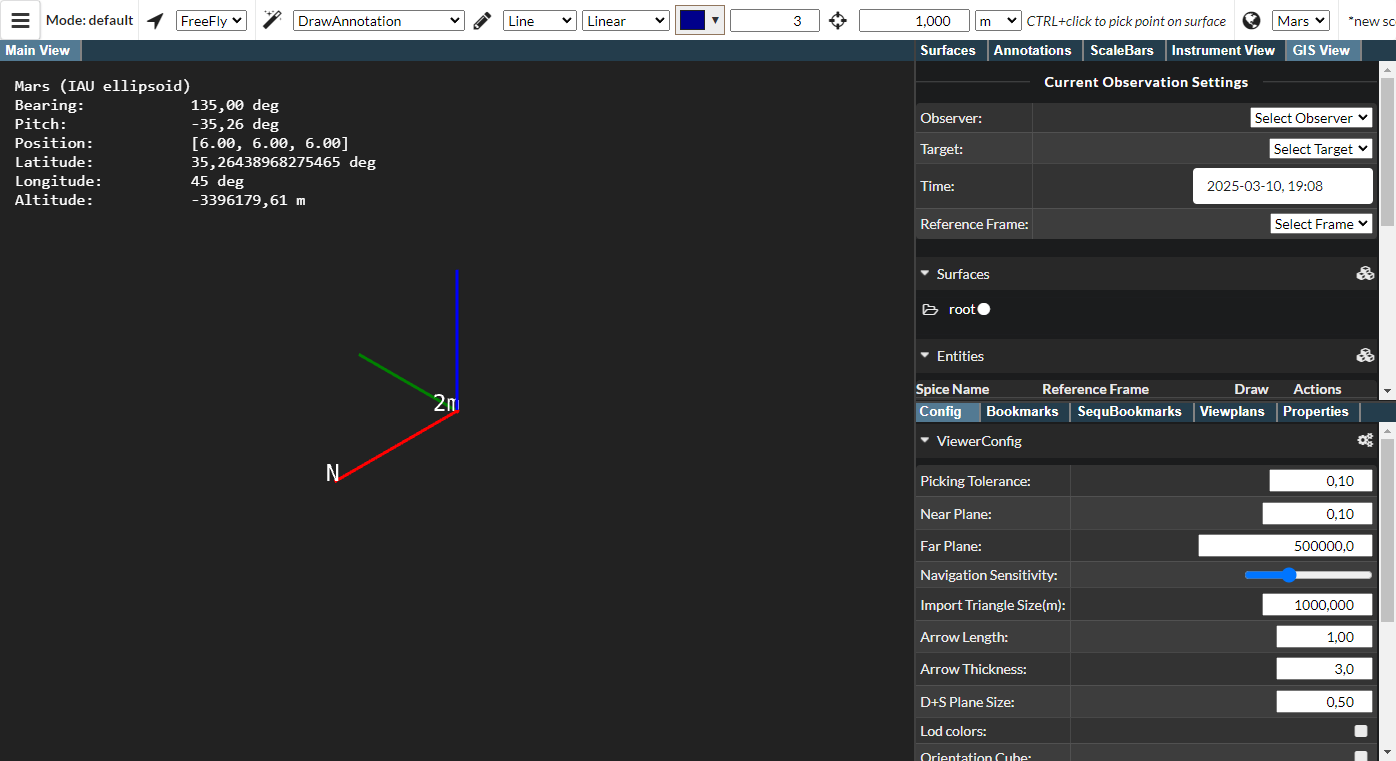
\includegraphics[width=0.8\textwidth]{./pics/gis-view.png}
	\caption{PRo3D with GIS View}
\end{figure}

\begin{enumerate}
	\def\labelenumi{\arabic{enumi}.}
	\setcounter{enumi}{1}
	\tightlist
	\item
	Load the kernel via:
\end{enumerate}

\begin{figure}[h!]
	\centering
	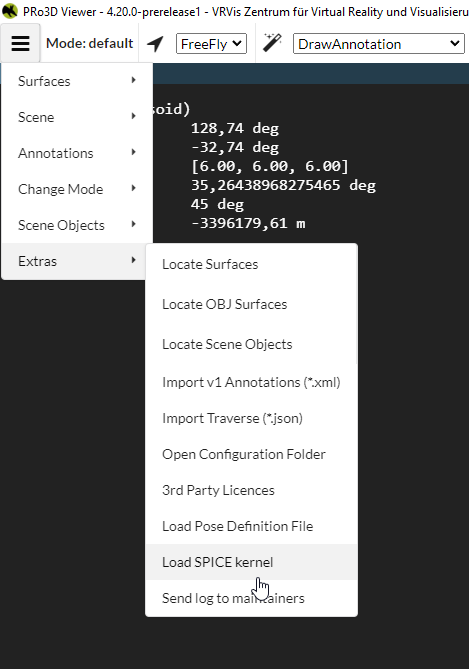
\includegraphics[width=0.4\textwidth]{pics/loadKernel.png}
	\caption{Loading the spice kernel.}
\end{figure}



\begin{enumerate}
	\def\labelenumi{\arabic{enumi}.}
	\setcounter{enumi}{2}
	\tightlist
	\item
	Then the Gis View should print the path to the kernel. Scroll down,
	and look at the settings pane within the GIS view.
\end{enumerate}

\begin{figure}[h!]
	\centering
	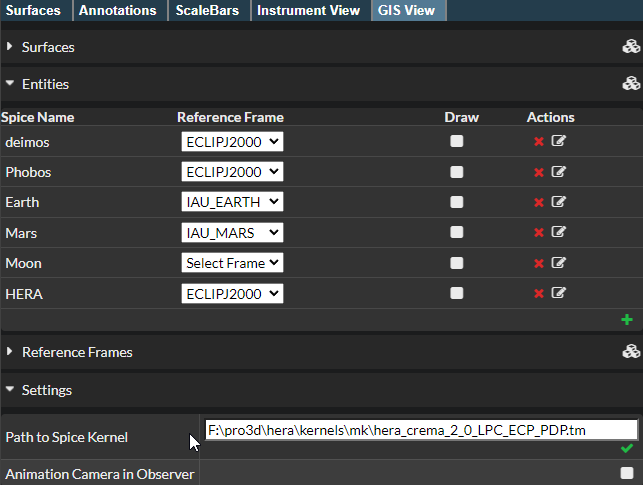
\includegraphics[width=0.8\textwidth]{pics/loadedKernel.png}
	\caption{Kernel Path in the GIS View.}
\end{figure}

A green check mark appears below the path if loading the kernel was
successful. If there is a red exclamation mark beneath the path loading
was not successful. PRo3D's text output will give more detailed
information why, it might be that the path to the kernel is not correct.

\hypertarget{pro3d-gis-view-tab}{%
	\subsubsection{PRO3D GIS View Tab}\label{pro3d-gis-view-tab}}

\hypertarget{current-observation-settings}{%
	\textbf{Current Observation
		Settings}\label{current-observation-settings}}

At the top of the GIS tab there is a section entitled ``Current
Observation Settings''. This is used to define the observed target, a camera location, a
point in time, and a reference frame.

\begin{figure}[h!]
	\centering
	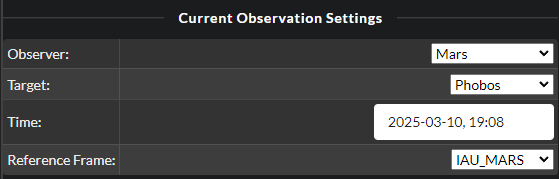
\includegraphics[width=0.8\textwidth]{pics/currentObservationSettings.png}
	\caption{Current Observation Settings.}
\end{figure}

\begin{itemize}
	\tightlist
	\item
	Observed body: The entity from which we want to observe a specific target.
	The camera will focus the observed body (look at it).
	\item
	Target: The entity we want to look at. The camera will look in the
	direction of the target.
	\item
	Time: The point of time at which we want to observe. The loaded spice
	kernel needs to have data for observer and target at the selected
	point in time!
	\item
	Reference Frame: The reference frame into which all other frames will
	be converted. Which frame is selected here should not change the
	visual result (except for trajectories).
\end{itemize}

\hypertarget{surfaces}{%
	\textbf{Surfaces}\label{surfaces}}

To use a surface with PRo3D's GIS functionality, it has to be associated
with a reference frame, and can be associated with an entity. This
reference frame in which the surface is defined is needed to transform
the surface to the global reference system used by PRo3D. Assigning a
reference frame and entity to a loaded surfaces is done in the
``Surfaces'' tab.

\begin{figure}[h!]
	\centering
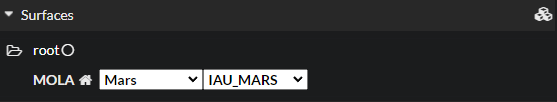
\includegraphics[width=1\textwidth]{pics/surfaces.png}
	\caption{Surfaces in the GIS view.}
\end{figure}


Select the correct reference frame (and optionally entity) from the
dropdown menu. If the entity or reference frame needed is not in the
dropdown menu, it can be created in the ``Entities''/``Reference
Frames'' tab.
\\

\hypertarget{entities}{%
	\textbf{Entities}\label{entities}}

Entities can be celestial bodies or spacecraft. To work with PRo3D's GIS
functionality the Spice Name of the entity needs to be defined in the
loaded spice kernel.

The entity tab lists all entities. There are some default entities
already present in PRo3D.

\begin{figure}[h!]
	\centering
	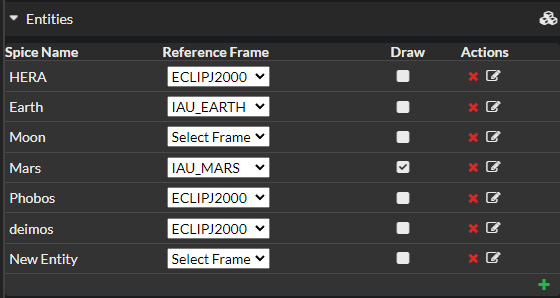
\includegraphics[width=0.6\textwidth]{pics/entities.png}
	\caption{Entities in the GIS view.}
\end{figure}



An entity can be edited by clicking on the right hand icon in the
``Actions'' column. The icon used to edit the HERA entity is circled in
red in the screenshot below.

\begin{figure}[h!]
	\centering
	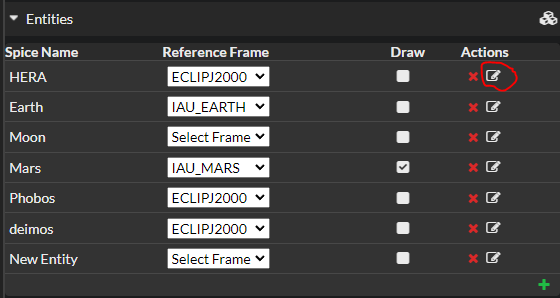
\includegraphics[width=0.6\textwidth]{pics/editEntities.png}
	\caption{Editing Entities.}
\end{figure}

The red cross to the left of the edit icon deletes the corresponding
entity.

Each entity can be assigned a reference frame in the column ``Reference
Frame''. For each entity, a sphere can be drawn in the scene. Whether a
sphere is drawn is determined by the checkbox in the ``Draw'' column.

A new entity can be created by clicking on the green plus icon at the
bottom right hand side of the Entities tab. The spice name can only be
set when creating an entity, it cannot be changed once the entity is
created. To change a spice name you need to deleted the old entity and
create a new one with the new spice name and the settings of the old
entity. Spice names are unique, so you cannot create two entities with
the same spice name.

Clicking on the edit icon of an entity (see above), opens a section for
the entity:

\begin{figure}[h!]
	\centering
	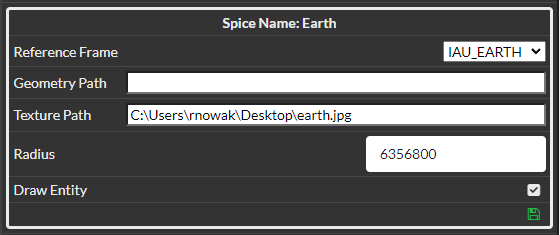
\includegraphics[width=0.6\textwidth]{pics/editEntity.png}
	\caption{Editing Entities.}
\end{figure}

The reference frame and whether to draw an entity can be selected in
this view as well as the following settings:

\begin{itemize}
	\tightlist
	\item
	\textbf{Geometry Path} (not yet implemented) path to a geometry that
	is displayed at the location of this entity instead of a simple sphere
	\item
	\textbf{Texture Path} The path to an image (for example a jpeg file)
	that is rendered onto the entity.
	\item
	\textbf{Radius} The radius of the sphere that is drawn in the location
	of the entity in meters.
\end{itemize}

The green save icon at the bottom right hand corner closes the edit
view.

Below an example of the entity Moon with a radius of 1736000 meters and
a texture path.

\begin{figure}[h!]
	\centering
	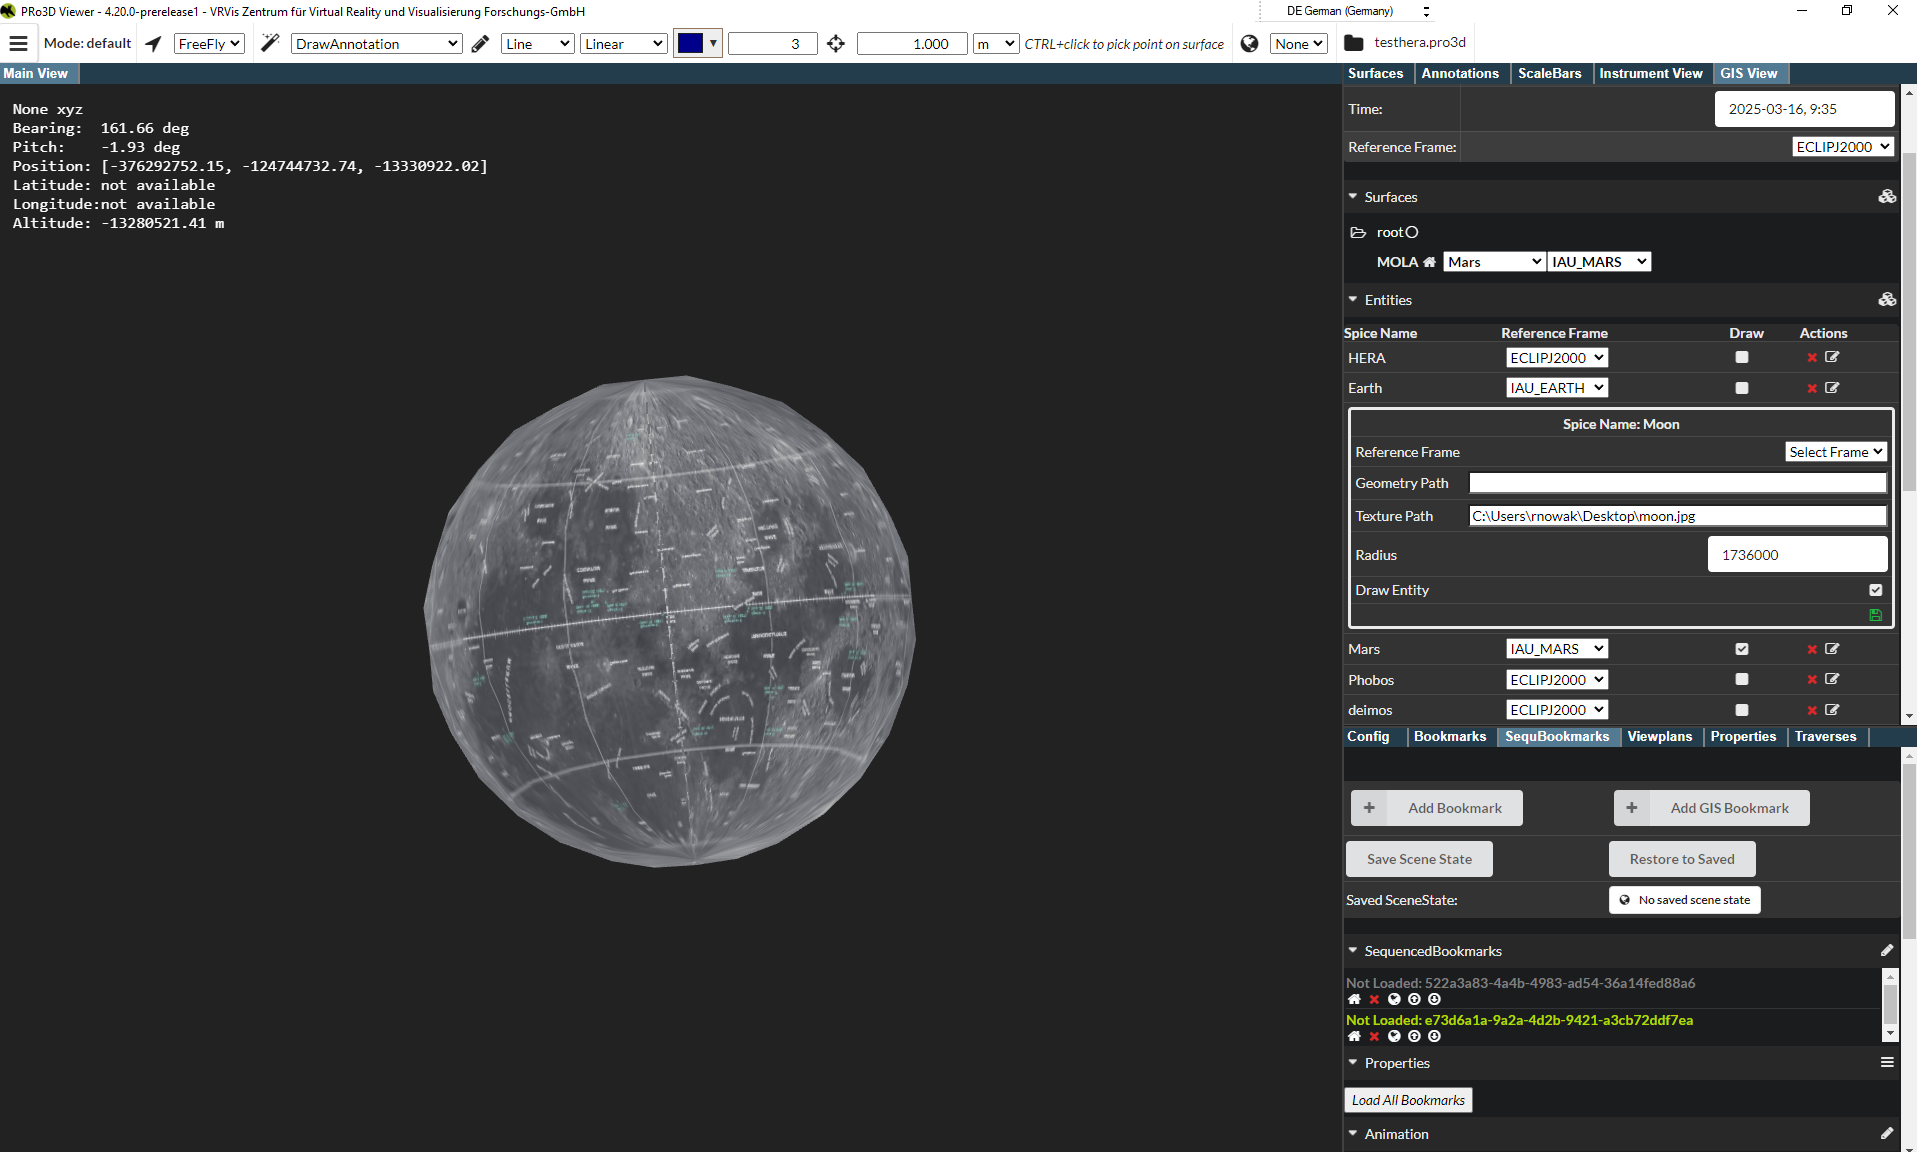
\includegraphics[width=1\textwidth]{pics/exampleMoonTexture.png}
	\caption{Textured Moon.}
\end{figure}



\hypertarget{reference-frames}{%
	\subsubsection{Reference Frames}\label{reference-frames}}

Reference frames can be deleted (red cross icon) and created (green plus
icon in the bottom right corner) in this view. They can also be assigned
an entity which is associated with them.

\begin{figure}[h!]
	\centering
	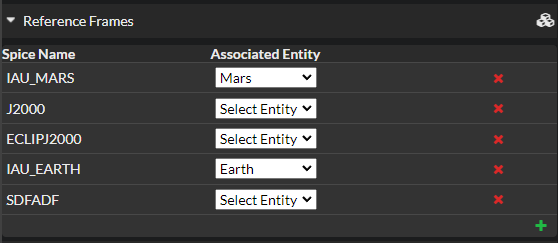
\includegraphics[width=0.6\textwidth]{pics/referenceFrames.png}
	\caption{Reference Frames.}
\end{figure}

A new reference frame can be created by clicking on the green plus icon
at the bottom right hand side of the Reference Frames tab. The spice
name can only be set when creating a reference frame, it cannot be
changed once the reference frame is created. To change a spice name you
need to deleted the old reference frame and create a new one with the
new spice name and the settings of the old reference frame. Spice names
are unique, so you cannot create two reference frame with the same spice
name.

\hypertarget{observing-mars}{%
	\subsubsection{Observing mars}\label{observing-mars}}

Let us now observe mars from, say phobos.

1. Set the observation settings (including a time which is in available in the kernel)

\begin{figure}[h!]
	\centering
	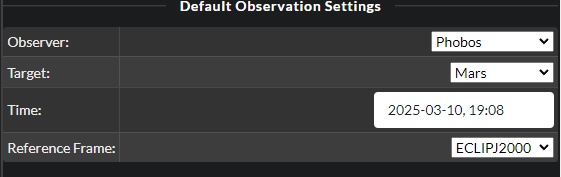
\includegraphics[width=0.6\textwidth]{pics/observe.png}
	\caption{Observing Settings.}
\end{figure}

2. Next, make sure the proxy visualization for mars is enabled:

\begin{figure}[h!]
	\centering
	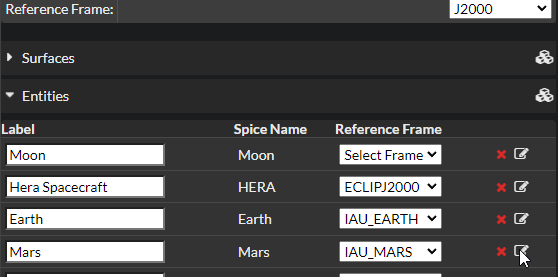
\includegraphics[width=0.6\textwidth]{./pics/MarsProperties.png}
	\caption{Proxy visualization for mars is enabled.}
\end{figure}

\begin{figure}[h!]
	\centering
	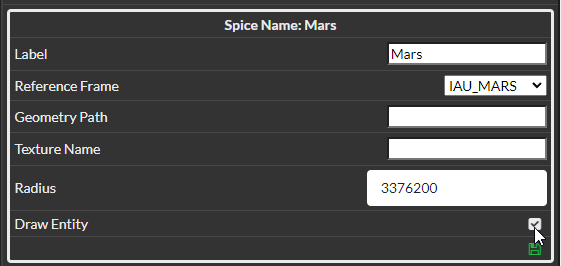
\includegraphics[width=0.6\textwidth]{./pics/visibleMars.png}
	\caption{Mars is now visible.}
\end{figure}

Also make sure to have the far plane set far away for viewing mars from
phobos. Ajust the near \emph{and} far planes accordingly.

\begin{figure}[h!]
	\centering
	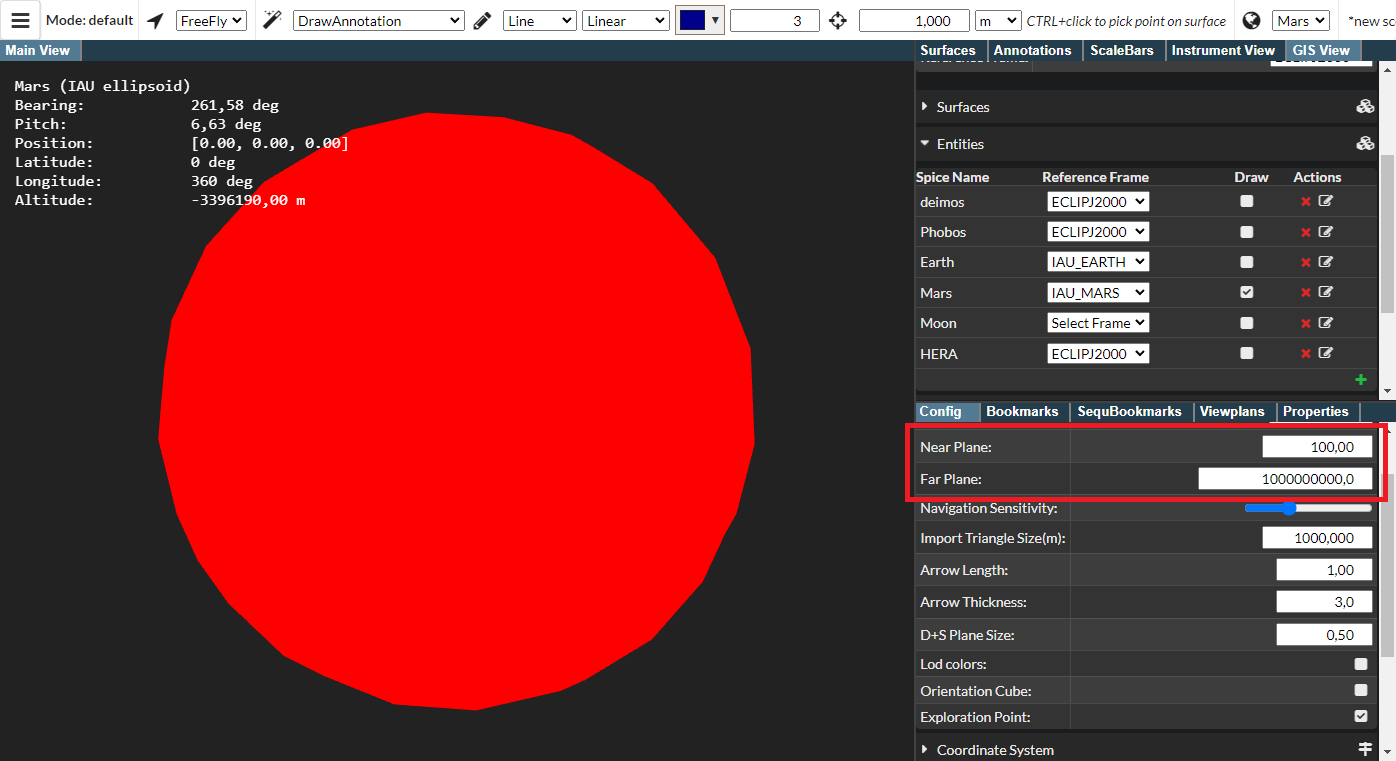
\includegraphics[width=1\textwidth]{./pics/farplane.png}
	\caption{The far plane needs to be set far enough away so objects are visible.}
\end{figure}

Now mars should be visible from the observation point of view.

By using the visualization properties in the entity list the element can
be textured as well.

\begin{figure}[h!]
	\centering
	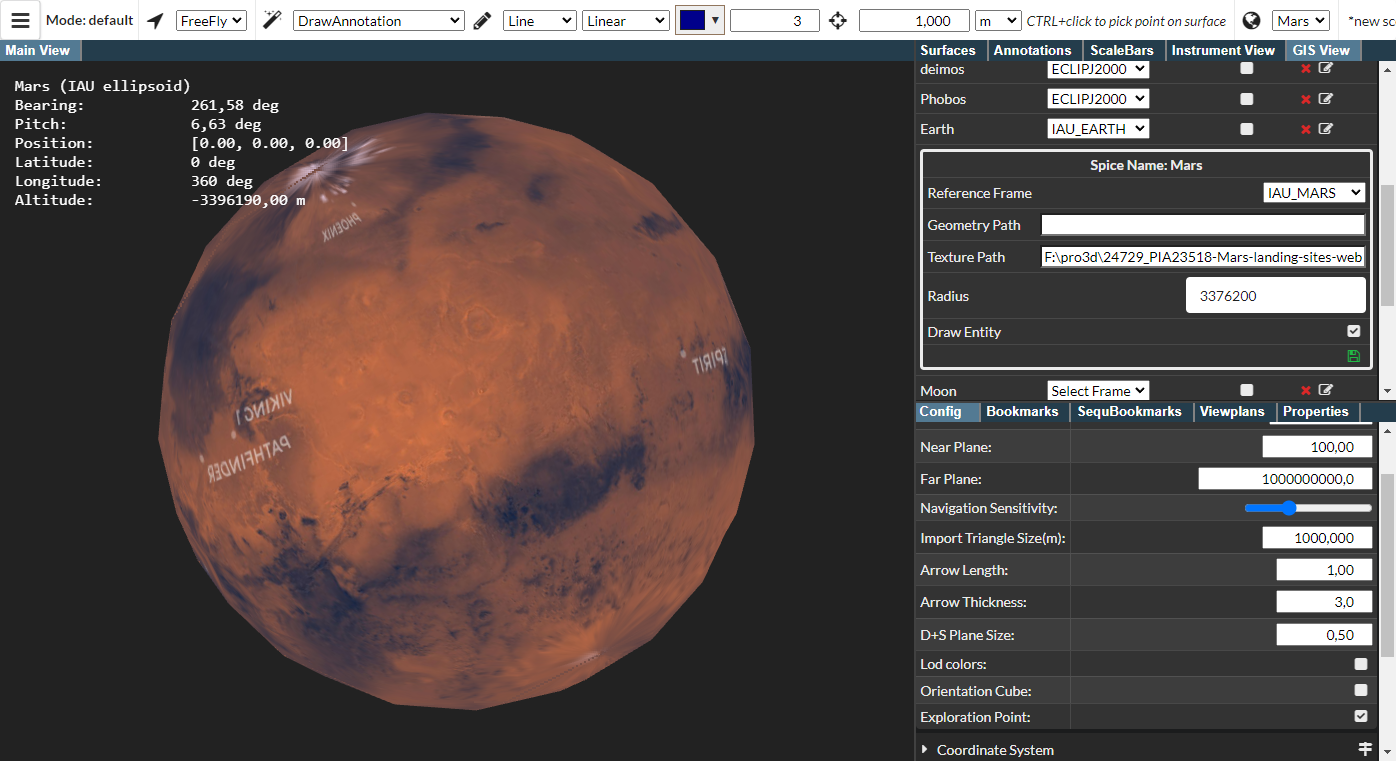
\includegraphics[width=1\textwidth]{./pics/textured.png}
	\caption{Textures can be specified and mapped onto entities.}
\end{figure}

Next let us load the mola dataset. In the Surfaces pane witin the Gis
View, now specifiy reference frame and celestial body for the surface
(if it does not appear change the observation settings, e.g.~by setting
the time).

\begin{figure}[h!]
	\centering
	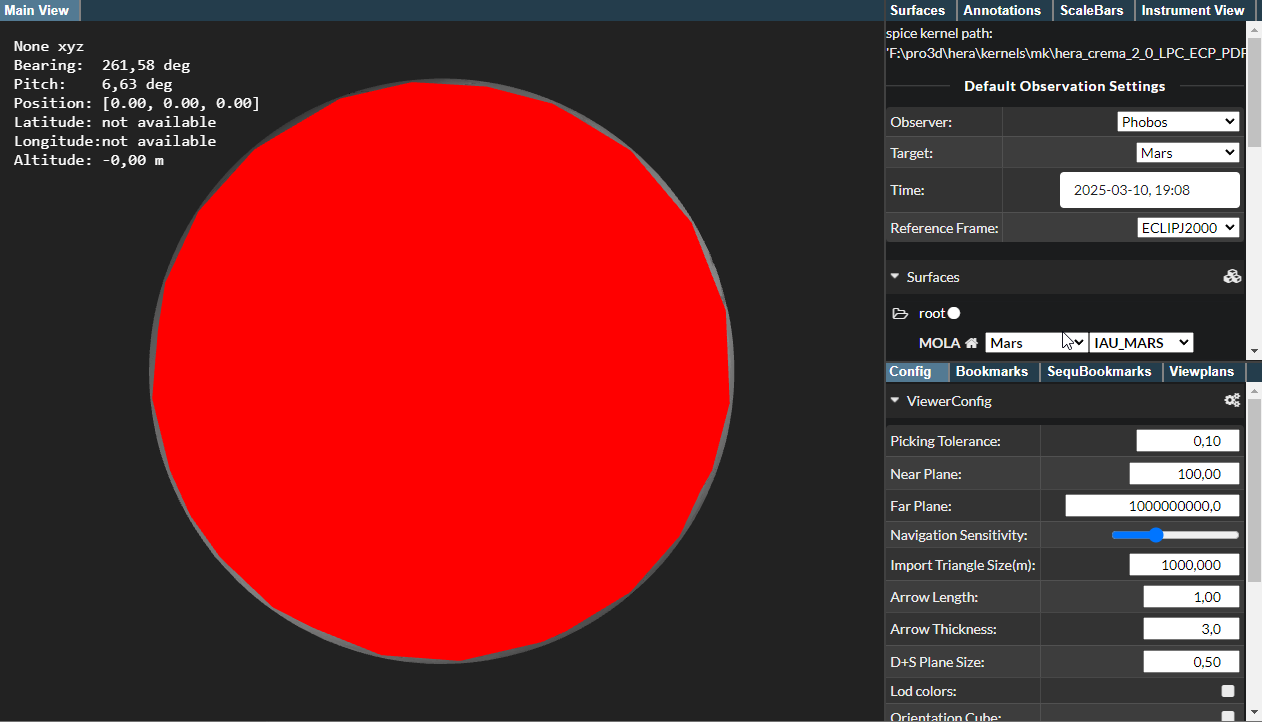
\includegraphics[width=1\textwidth]{pics/surfaceRefFrame.png}
	\caption{Specifiy reference frame and celestial body.}
\end{figure}

Since we have a full surface for mars now, we can switch off the proxy
geometry:

\begin{figure}[h!]
	\centering
	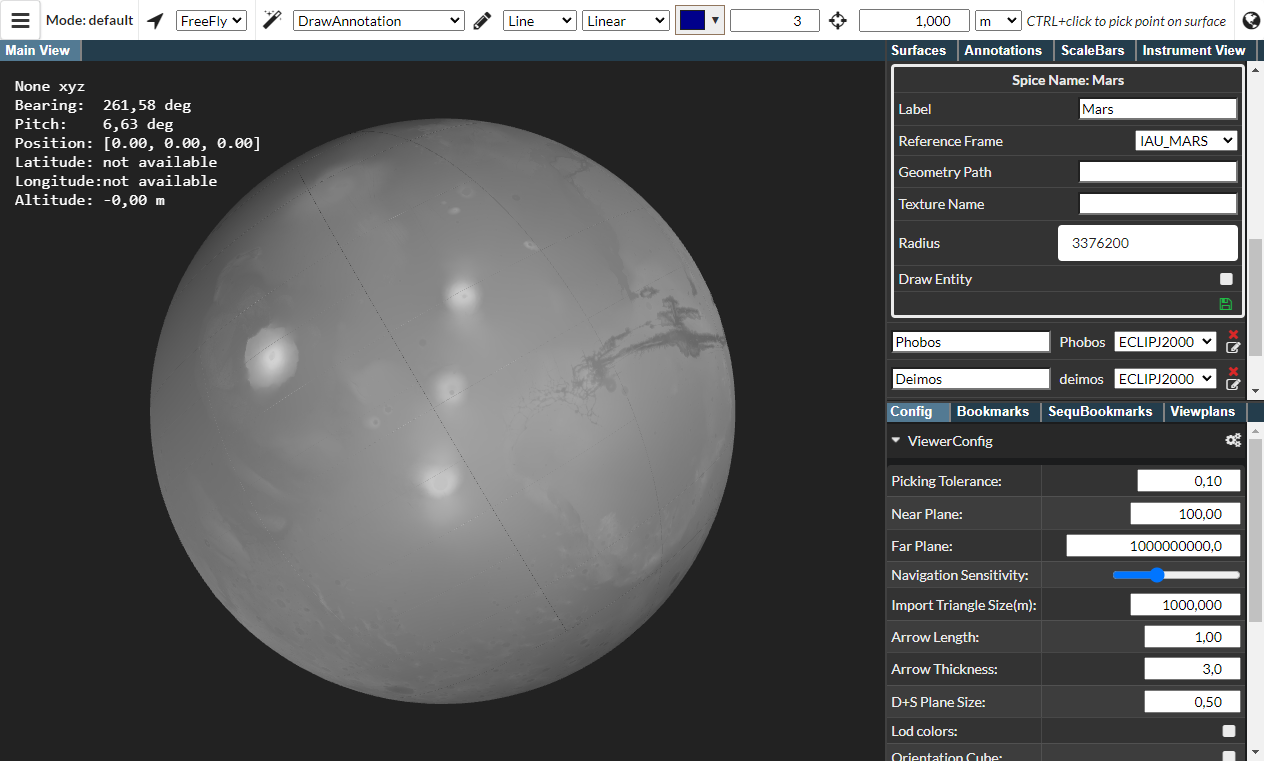
\includegraphics[width=1\textwidth]{pics/molaObservation.png}
	\caption{After switching off the proxy geometry, the loaded OPC is visible.}
\end{figure}

\newpage

\hypertarget{extended-features}{%
	\subsubsection{Extended features}\label{extended-features}}

It is possible to add new celestial bodies, new reference frames.

\hypertarget{extended-concept}{%
	\subsubsection{Extended concept}\label{extended-concept}}

For story telling, PRo3D also supports to create GIS bookmarks.
Similarly to stories on surfaces this can be used to create movies and
interactive presentations for science.

\hypertarget{caveats}{%
	\subsubsection{Caveats}\label{caveats}}

Currently the GIS settings are not stored to scene files.

%----------------------------------------------------------------------------------------
%	SubSection: 
%----------------------------------------------------------------------------------------
\newpage
\subsection{Contour Lines}
\label{sec:contourLines}

\begin{figure}[h!]
	\centering
	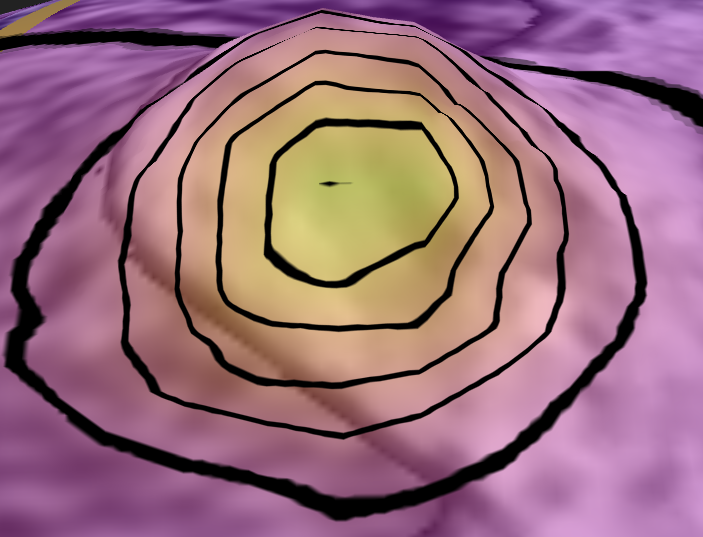
\includegraphics[width=0.8\textwidth]{pics/contourTeaser.png}
	\caption{The contour lines feature.}
\end{figure}

The feature only works in combination with multilayer opcs. By using surface properties, choose a particular layer as a secondary texture:

\begin{figure}[h!]
	\centering
	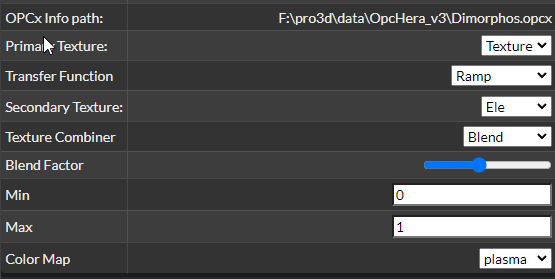
\includegraphics[width=0.6\textwidth]{pics/multitexture-ui.png}
	\caption{The multitexture UI.}
\end{figure}

Next, in the contour section, enable it and set distance of the lines, as well as line width and line border (both in the domain of the value chosen for texturing, here `Ele`).

\begin{figure}[h!]
	\centering
	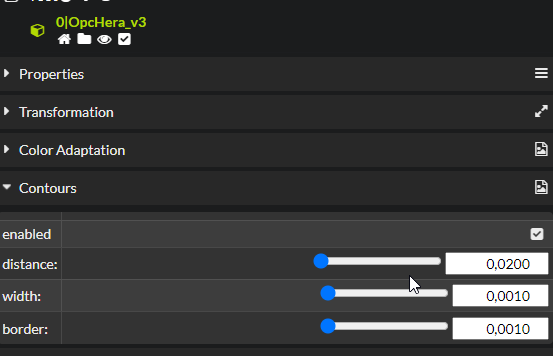
\includegraphics[width=0.6\textwidth]{pics/contour1.png}
	\caption{In the contour section, enable it and set distance of the lines, as well as line width and line border.}
\end{figure}

\begin{figure}[h!]
	\centering
	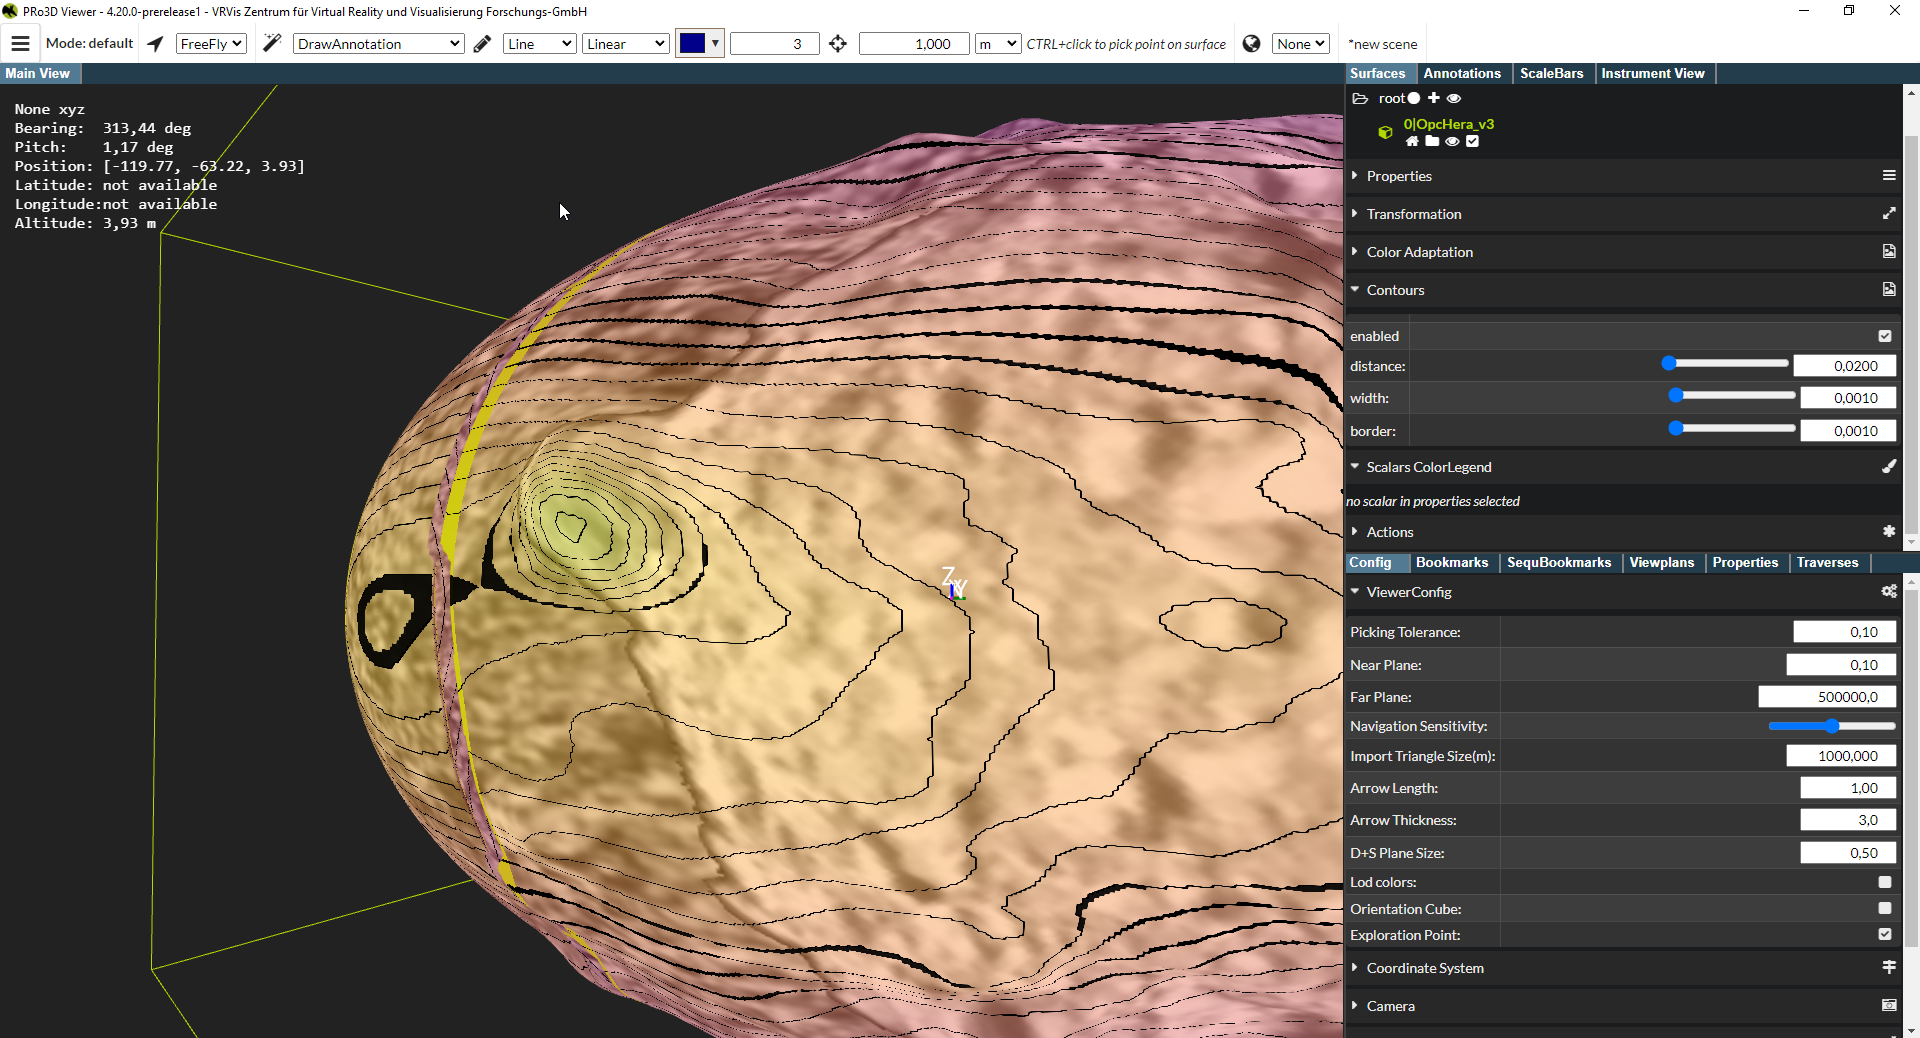
\includegraphics[width=1.0\textwidth]{pics/contour0.png}
	\caption{The whole setup looks like this.}
\end{figure}

%----------------------------------------------------------------------------------------
%	SubSection: 
%----------------------------------------------------------------------------------------

\clearpage

\subsection{Multitexturing}
\label{sec:multitexturing}

This feature allows to visualize multiple (opc) texture layers and control visualization properties.

Instrument data and reconstruction information for example can be mapped onto the surface and blended with the albedo texture (here an accuracy map of the reconstruction):

\begin{figure}[h!]
	\centering
	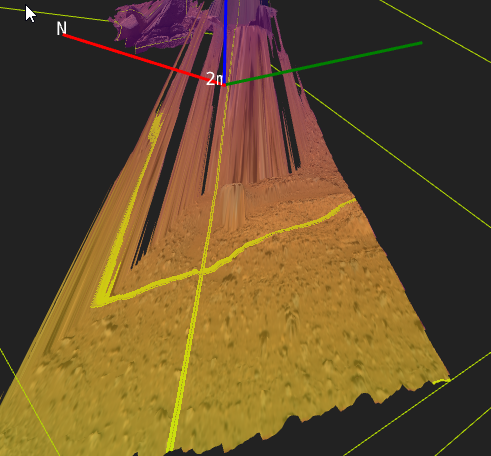
\includegraphics[width=0.6\textwidth]{pics/AccuracyMap.png}
	\caption{An accuracy map of the reconstruction.}
\end{figure}

By using query parameters and a transfer function specific attributes can be filtered (e.g. here the elevation):

\begin{figure}[h!]
	\centering
	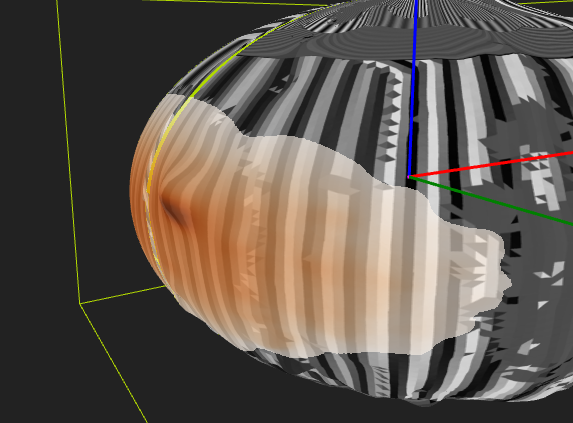
\includegraphics[width=0.6\textwidth]{pics/FilteredElevation.png}
	\caption{The elevation is filtered.}
\end{figure}

The controls can be found in the surface properties when selecting a surface. 

\begin{figure}[h!]
	\centering
	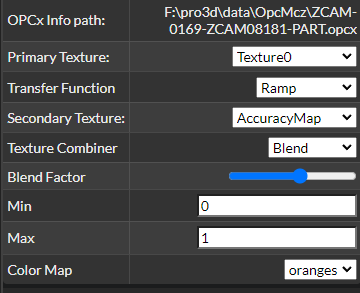
\includegraphics[width=0.6\textwidth]{pics/MultitexControls.png}
	\caption{The multitexturing controls in the surface properties.}
\end{figure}

\paragraph{Caveats and missing features}
Currently we only read opcx files as opposed to opcx.json files which also provide a friendly name for the texture layers. In favor of reduced complexity we opted for the simpler, established opcx solution which could also be extended to contain a friendly name for the layer.

\paragraph{Data Example}
An example of currently available data can be found in the Appendix \ref{multitexturingAppendix}.


